\documentclass[10pt,a4paper]{article}
\usepackage[utf8]{inputenc}
\usepackage{amsmath}
\usepackage{amsfonts}
\usepackage{amssymb}
\usepackage{booktabs}
\usepackage{tikz}
\usepackage{adjustbox}
\usepackage{caption}  
\usetikzlibrary{positioning,angles,quotes,calc,shapes}
\begin{document}










\section{Notation and Modeling for Classed Jackson Networks}



\begin{table}
\caption{Tempi esecuzione sperimentali (espessi in $\mu s$) ottenuti da vari test}\label{table:diana}
\begin{center}
\begin{tabular}{cc}

\toprule

$\lambda_{controller}(1)$ & Total mean arrival rate into \textit{controller} of class $1$ tasks \\
$\lambda_{controller}(2)$ & Total mean arrival rate into \textit{controller} of class $2$ tasks \\
$\mu_{cloudlet}(1)$ & Mean service rate at \textit{cloudlet} of class $1$ tasks \\
$\mu_{cloudlet}(2)$ & Mean service rate at \textit{cloudlet} of class $2$ tasks \\
$\mu_{cloud}(1)$ & Mean service rate at \textit{cloud} of class $1$ tasks \\
$\mu_{cloud}(2)$ & Mean service rate at \textit{cloud} of class $2$ tasks \\
\end{tabular}
\end{center}
\end{table}

\newpage
\section{Analytical solution}

In this last section we will develop an analytical solution to validate the results obtained previously through our simulations.

\subsection{System based on access control Algorithm 1}
\begin{figure}
\caption{Cloudlet system component modeled using a CTMC} \label{fig:CloudletMarkovChain}
\begin{adjustbox}{center=\textwidth}
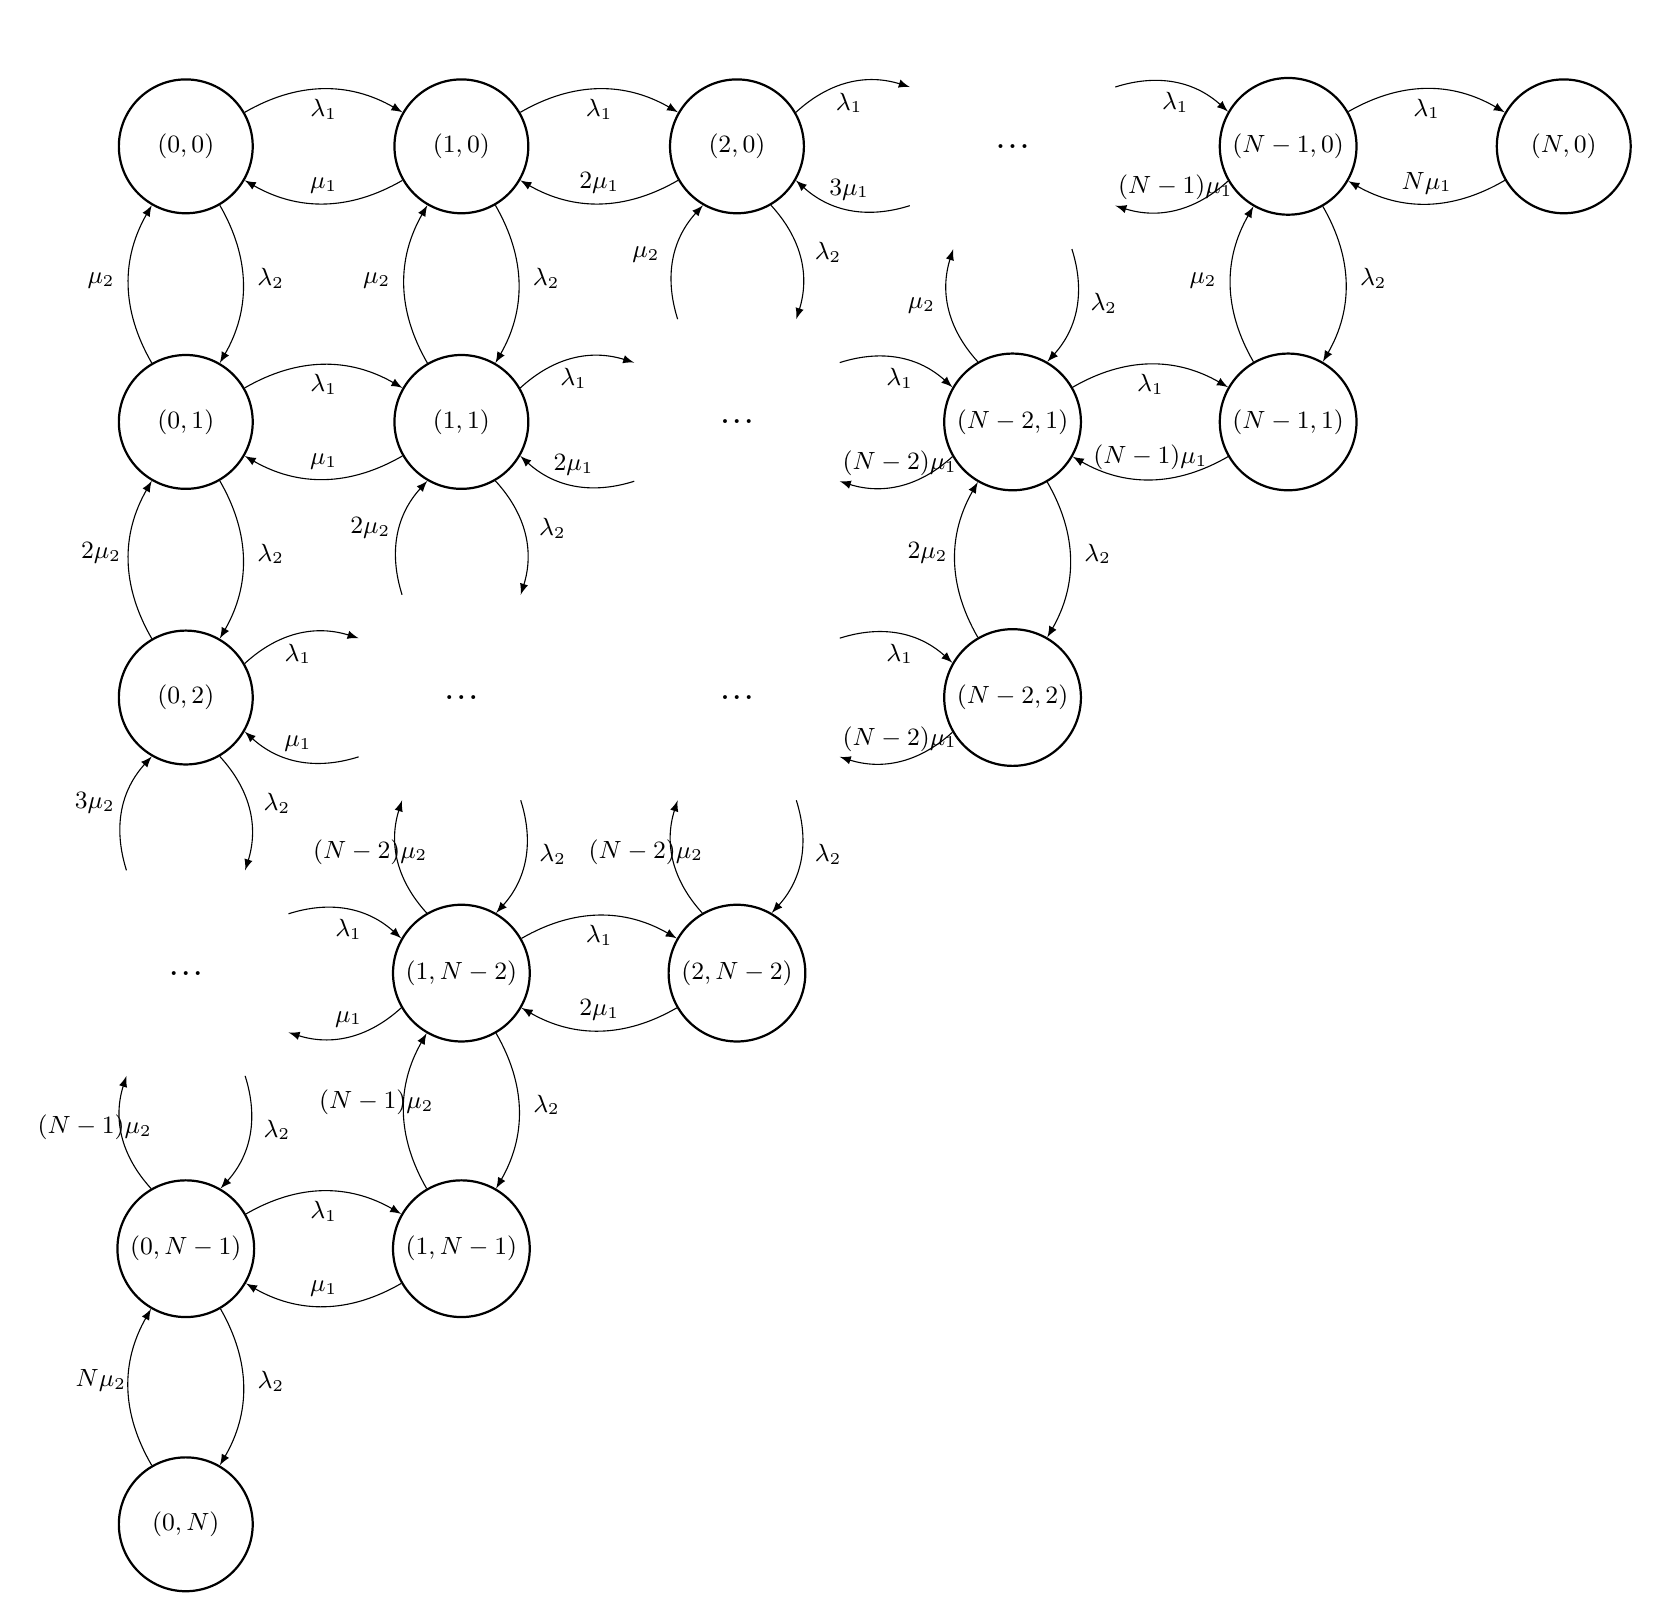
\begin{tikzpicture}[->,node distance=3.5cm,>=latex,font=\small, minimum width=1.7cm]

    \tikzstyle{round}=[thick,draw=black,circle]

    \node[round] 			    (00) {$(0,0)$};
    \node[round,right of=00]    (10) {$(1,0)$};
    \node[round,below of=00]    (01) {$(0,1)$};
    \node[round,below of=10]    (11) {$(1,1)$};
    \node[round,below of=01]    (02) {$(0,2)$};
    \node[round,right of=10]    (20) {$(2,0)$};
   
    \node[circle,draw=white,right of=20, minimum width = 3cm]    (A1) {\LARGE ...};
    \node[circle,draw=white,below of=02, minimum width = 3cm]    (A2) {\LARGE ...};
     
   	\node[round,right of=A1]    (N-1/0)  	{$(N-1,0)$};
   	\node[round,right of=N-1/0] (N0)	 	{$(N,0)$};
    \node[round,below of=N-1/0] (N-1/1)     {$(N-1,1)$};
    \node[round,left  of=N-1/1] (N-2/1)	{$(N-2,1)$};
    \node[round,below of=N-2/1] (N-2/2)	{$(N-2,2)$};
   
    \node[round,below of=A2]    (0/N-1)  	{$(0,N-1)$};
   	\node[round,below of=0/N-1] (0N)	 	{$(0,N)$};
    \node[round,right of=0/N-1] (1/N-1)     {$(1,N-1)$};
    \node[round,above of=1/N-1] (1/N-2)     {$(1,N-2)$};
    \node[round,right of=1/N-2] (2/N-2)	    {$(2,N-2)$};
    
    
    \node[circle,draw=white,left of=N-2/1,minimum width = 3cm]        (A3)     {\LARGE ...};
    \node[circle,draw=white,below of=11,minimum width = 3cm]          (A4)     {\LARGE ...};
    \node[circle,draw=white,above of=2/N-2,minimum width = 3cm]       (A5)     {\LARGE ...};
 
 
 	\path 
 	(00) 	edge[bend left,below]		node 					    {$\lambda_1$}		(10)
 		 	edge[bend left,above]       node [xshift=10,yshift=-5]  {$\lambda_2$} 		(01)
 	
 	(10) 	edge[bend left,above]       node 						{$\mu_1$} 			(00)
 		 	edge[bend left,below]		node 					    {$\lambda_1$}		(20)
 		 	edge[bend left,above]       node [xshift=10,yshift=-5]  {$\lambda_2$} 		(11)
 	
    (01) 	edge[bend left,above]       node [xshift=-10,yshift=-5] {$\mu_2$} 			(00)
   		 	edge[bend left,below]		node 					    {$\lambda_1$}		(11)
   	     	edge[bend left,above]       node [xshift=10,yshift=-5]  {$\lambda_2$} 		(02)
   
    (20) 	edge[bend left,above]       node 						{$2\mu_1$} 			(10)
    		edge[bend left,below]		node 					    {$\lambda_1$}		(A1)
    		edge[bend left,above]       node [xshift=10,yshift=-5]  {$\lambda_2$} 		(A3)
   		    
    (02) 	edge[bend left,above]       node [xshift=-10,yshift=-5] {$2\mu_2$} 			(01)
    		edge[bend left,above]       node [xshift=10,yshift=-5]  {$\lambda_2$} 		(A2)
    		edge[bend left,below]		node 					    {$\lambda_1$}		(A4)
   
    (11) 	edge[bend left,above]       node [xshift=-10,yshift=-5] {$\mu_2$} 			(10)
   		 	edge[bend left,above]       node 						{$\mu_1$} 			(01)
   		 	edge[bend left,below]		node 					    {$\lambda_1$}		(A3)
   		 	edge[bend left,above]       node [xshift=10,yshift=-5]  {$\lambda_2$} 		(A4)
   
   	(N0) 	edge[bend left,above]       node 						{$N\mu_1$} 			(N-1/0)
   
   	(N-1/0) edge[bend left,below]		node 					    {$\lambda_1$}		(N0)
   			edge[bend left,above]       node [xshift=10,yshift=-5]  {$\lambda_2$} 		(N-1/1)
   			edge[bend left,above]       node 						{$(N-1)\mu_1$} 			(A1)
   
    (N-1/1) edge[bend left,above]       node [xshift=-10,yshift=-5] {$\mu_2$} 			(N-1/0)
    		edge[bend left,above]       node 						{$(N-1)\mu_1$} 		(N-2/1)
    
    (N-2/1) edge[bend left,below]		node 					    {$\lambda_1$}		(N-1/1)
    		edge[bend left,above]       node [xshift=-10,yshift=-5] {$\mu_2$} 			(A1)
    		edge[bend left,above]       node 						{$(N-2)\mu_1$} 		(A3)
    		edge[bend left,above]       node [xshift=10,yshift=-5]  {$\lambda_2$} 		(N-2/2)
    		
    (N-2/2) edge[bend left,above]       node [xshift=-10,yshift=-5] {$2\mu_2$} 			(N-2/1)
    		edge[bend left,above]       node 						{$(N-2)\mu_1$} 		(A5)
    
    (0N) 	edge[bend left,above]       node [xshift=-10,yshift=-5]	{$N\mu_2$} 			(0/N-1)
   
   	(0/N-1) edge[bend left,below]		node 					    {$\lambda_1$}		(1/N-1)
   			edge[bend left,above]       node [xshift=10,yshift=-5]  {$\lambda_2$} 		(0N)
   			edge[bend left,above]       node [xshift=-10,yshift=-5]	{$(N-1)\mu_2$} 		(A2)
   
    (1/N-1) edge[bend left,above]       node 						{$\mu_1$}  			(0/N-1)
    	    edge[bend left,above]       node [xshift=-10,yshift=-5]	{$(N-1)\mu_2$} 		(1/N-2)
    
    (1/N-2) edge[bend left,above]       node 						{$\mu_1$}  			(A2)
    		edge[bend left,above]       node [xshift=10,yshift=-5]  {$\lambda_2$} 		(1/N-1)
    		edge[bend left,above]       node [xshift=-10,yshift=-5]	{$(N-2)\mu_2$} 		(A4)
    		edge[bend left,below]		node 					    {$\lambda_1$}		(2/N-2)
    		
    (2/N-2) edge[bend left,above]       node 						{$2\mu_1$}  		(1/N-2)
    		edge[bend left,above]       node [xshift=-10,yshift=-5]	{$(N-2)\mu_2$} 		(A5)
    
    (A1)    edge[bend left,above]       node 						{$3\mu_1$} 			(20)
    	    edge[bend left,below]		node 					    {$\lambda_1$}		(N-1/0)
    	    edge[bend left,above]       node [xshift=10,yshift=-5]  {$\lambda_2$} 		(N-2/1)
    	    
    (A2)	edge[bend left,above]       node [xshift=10,yshift=-5]  {$\lambda_2$} 		(0/N-1)
    		edge[bend left,above]       node [xshift=-10,yshift=-5]	{$3\mu_2$} 			(02)
    		edge[bend left,below]		node 					    {$\lambda_1$}		(1/N-2)
    		
    (A3)    edge[bend left,below]		node 					    {$\lambda_1$}		(N-2/1)
    		edge[bend left,above]       node [xshift=-10,yshift=-5]	{$\mu_2$} 			(20)
    		edge[bend left,above]       node 						{$2\mu_1$} 			(11)
    
    (A4)    edge[bend left,above]       node [xshift=-10,yshift=-5]	{$2\mu_2$} 			(11)
    		edge[bend left,above]       node 						{$\mu_1$} 			(02)
    		edge[bend left,above]       node [xshift=10,yshift=-5]  {$\lambda_2$} 		(1/N-2)
    		
    (A5)    edge[bend left,above]		node [xshift=10,yshift=-5]  {$\lambda_2$}		(2/N-2)
    		edge[bend left,below]		node 					    {$\lambda_1$}		(N-2/2);
   
\end{tikzpicture}
\end{adjustbox}
\end{figure}

In order to compute all parameters and metrics of interest associated with above-mentioned system \textbf{based on access control Algorithm 1}, is crucial to determine the \textbf{fraction of jobs that are forwarded to the cloud}. 

According to our model, the cloudlet has limited resources therefore he can accept jobs until their number does not exceed a given threshold $N$; the key point is to compute the probability according to which the sum of job of each class in cloudlet system is equal to that threshold. 

Formally, we can determine this probability by modelling the cloudlet system as \textbf{continuous-time Markov chain} (\textbf{CTMC}), of which a graphical representation is shown in Figure \ref{fig:CloudletMarkovChain}, where the state, denoted with $(n_1,n_2)$, corresponds to the number of class 1 job $n_1$ and class 2 job $n_2$ present in system at a certain moment.

Obviously we can compute \textbf{limiting probabilities}, namely the probability according to which the chain is in a state $j$ independently of the starting state, for each states of the Cloudlet CTMC by solving the \textbf{balance equations}, in which we can equate the rate at which the system leaves state $j$ with the rate at which the system enters state $j$.\footnote{\textit{Cfr.} Mor Harchol-Balter - \textit{Performance Modeling and Design of Computer Systems} - Carnegie Mellon University, Pennsylvania, pag. 237}

\paragraph{Balance equation computing} In order to compute $\pi_{(n1,n2)}$, we must resolve balance equations for given CTMC shown in Equation \ref{equation:AccessControlAlgorithm1-BalanceEquations}. Is important to remember that these equation, automatically generated through a very simple Java script fully described into \texttt{ALG-1-MATLAB-ScriptGenerator.java} file, have been resolved using a MATLAB\texttrademark  script, called \texttt{ALG-1-MATLAT-Script.m}.

\begin{adjustbox}{center=\textwidth}
\label{equation:AccessControlAlgorithm1-BalanceEquations}

$\begin{cases} 
(\lambda_1 + \lambda_2)\pi_{(0,0)} = \mu_1\pi_{(1,0)} + \mu_2\pi_{(0,1)} \\

(\lambda_1 + \lambda_2 + i\mu_1)\pi_{(i,0)} = \lambda_1\pi_{(i-1,0)} + \mu_1(i+1)\pi_{(i+1,0)} + \mu_2\pi_{(i,1)} & \forall i \in \mathbb{N} \mid 1 \leq i \leq N-1 \\

(\lambda_1 + \lambda_2 + i\mu_2)\pi_{(0,i)} = \lambda_2\pi_{(0,i-1)} + \mu_1\pi_{(1,i)} + \mu_2(i+1)\pi_{(0,i+1)} & \forall i \in \mathbb{N} \mid 1 \leq i \leq N-1 \\

\mu_1N\pi_{(N,0)} = \lambda_1\pi_{(N-1,0)} \\

\mu_2N\pi_{(0,N)} = \lambda_2\pi_{(0,N-1)} \\

(i\mu_1 + j\mu_2)\pi_{(i,j)} = \lambda_1\pi_{(i-1,j)} + \lambda_2\pi_{(i,j-1)} & \forall i,j \in \mathbb{N} \mid \begin{array} {l} 1 \leq i \leq N-1 \\ 1 \leq j \leq N-1 \end{array} \mid i + j = N \\

(\lambda_1 + \lambda_2 + i\mu_1 + j\mu_2)\pi_{(i,j)} = \lambda_1\pi_{(i-1,j)} + \lambda_2\pi_{(i,j-1)} + \mu_1(i+1)\pi_{(i+1,j)} + \mu_2(j+1)\pi_{(i,j+1)} & \forall i,j \in \mathbb{N} \mid \begin{array} {l} 1 \leq i \leq N-1 \\ 1 \leq j \leq N-1 \end{array} \mid i + j < N \\

\sum \pi_{(i,j)} = 1 & \forall i,j \in \mathbb{N}_0 \mid 

\end{cases}
$ 
\end{adjustbox}

\paragraph{Probabilities computing} ù

Having found the stationary probabilities, we now find the \textbf{probability that an arriving job has to be forwarded to cloud}, \textbf{$\Pi_A$}. Observe that:
\begin{itemize}
\item The class to which an arrival job belongs is not important for system based on access control Algorithm 1, that is we make no distinction between a class 1 or class 2 arrival job.
\item $\Pi_A$ is the probability that an arrival job find that the number of jobs present in cloudlet has exceeded given threshold $N$; that is occurs that $n_1 + n_2 = N$.
\end{itemize}

\begin{equation}
\begin{array} {lcl} 
\Pi_A & = & P\lbrace{\text{An arrival sees $N$ jobs in cloudlet}}\rbrace \\
& = & \text{Limiting probability that there are $N$ jobs in system} \\
& = & \displaystyle \sum_{\substack{ n1+n2=N \\ n_1, n_2 \in \mathbb{N}_0}} \pi(n_1,n_2)
\end{array}
\end{equation}










\begin{table}[h!]
    \centering
    \label{tab:MalwareFileList}
    \begin{tabular}{r|l}
     \toprule

      $r_i(c)$ & Outside arrival rate into server $i$ of class $c$ packets \\
      \hline
      $P_{ij}^{(c)}$ & Probability that when a packet of class $c$ finishes at server $i$, it next moves to server $j$ \\
      \hline
      $\lambda_i(c)$ & Total arrival rate into server i of class c packet \\ 
      \bottomrule
    \end{tabular}
\end{table}

\begin{equation}
\lambda_{\text{cloudlet}}(1) = \lambda_{\text{controller}}(1)\cdot P^{(1)}_{\text{controller,cloudlet}}
\end{equation}

\begin{equation}
\lambda_{\text{cloudlet}}(2) = \lambda_{\text{controller}}(2)\cdot P^{(2)}_{\text{controller,cloudlet}}
\end{equation}

\begin{equation}
\lambda_{\text{cloud}}(1) = \lambda_{\text{controller}}(1)\cdot P^{(1)}_{\text{controller,cloud}}
\end{equation}

\begin{equation}
\lambda_{\text{cloud}}(2) = \lambda_{\text{controller}}(2)\cdot P^{(2)}_{\text{controller,cloud}}
\end{equation}



\begin{equation}
P^{(1)}_{\text{controller,cloudlet}} = P^{(2)}_{\text{controller,cloudlet}} = 1 - \Pi
\end{equation}

For cloudlet:

\begin{equation}
\lambda_{\text{cloudlet}} = \lambda_{\text{cloudlet}}(1) + \lambda_{\text{cloudlet}}(2)
\end{equation}

\begin{equation}
\lambda_{\text{cloud}} = \lambda_{\text{cloud}}(1) + \lambda_{\text{cloud}}(2)
\end{equation}

contribution to the load due to jobs of priority 1:


\begin{equation}
\rho_{\text{cloudlet}}(1) = \dfrac{\lambda_{\text{cloudlet}}(1)}{\mu_{\text{cloudlet}}(1)} 
\end{equation}

\begin{equation}
\rho_{\text{cloudlet}}(2) = \dfrac{\lambda_{\text{cloudlet}}(2)}{\mu_{\text{cloudlet}}(2)} 
\end{equation}

\begin{equation}
\rho_{\text{cloud}}(1) = \dfrac{\lambda_{\text{cloud}}(1)}{\mu_{\text{cloud}}(1)} 
\end{equation}

\begin{equation}
\rho_{\text{cloud}}(2) = \dfrac{\lambda_{\text{cloud}}(2)}{\mu_{\text{cloud}}(2)} 
\end{equation}

.......


\begin{equation}
E[N_{\text{cloudlet}}(1)] = \dfrac{\rho_{\text{cloudlet}}(1)}{1 - \rho_{\text{cloudlet}}(1)}
\end{equation}

\subsection{System based on access control Algorithm 2}

\begin{figure}
\caption{Cloudlet system component modeled using a CTMC} \label{fig:ALG2-CloudletMarkovChain}
\begin{adjustbox}{center=\textwidth}
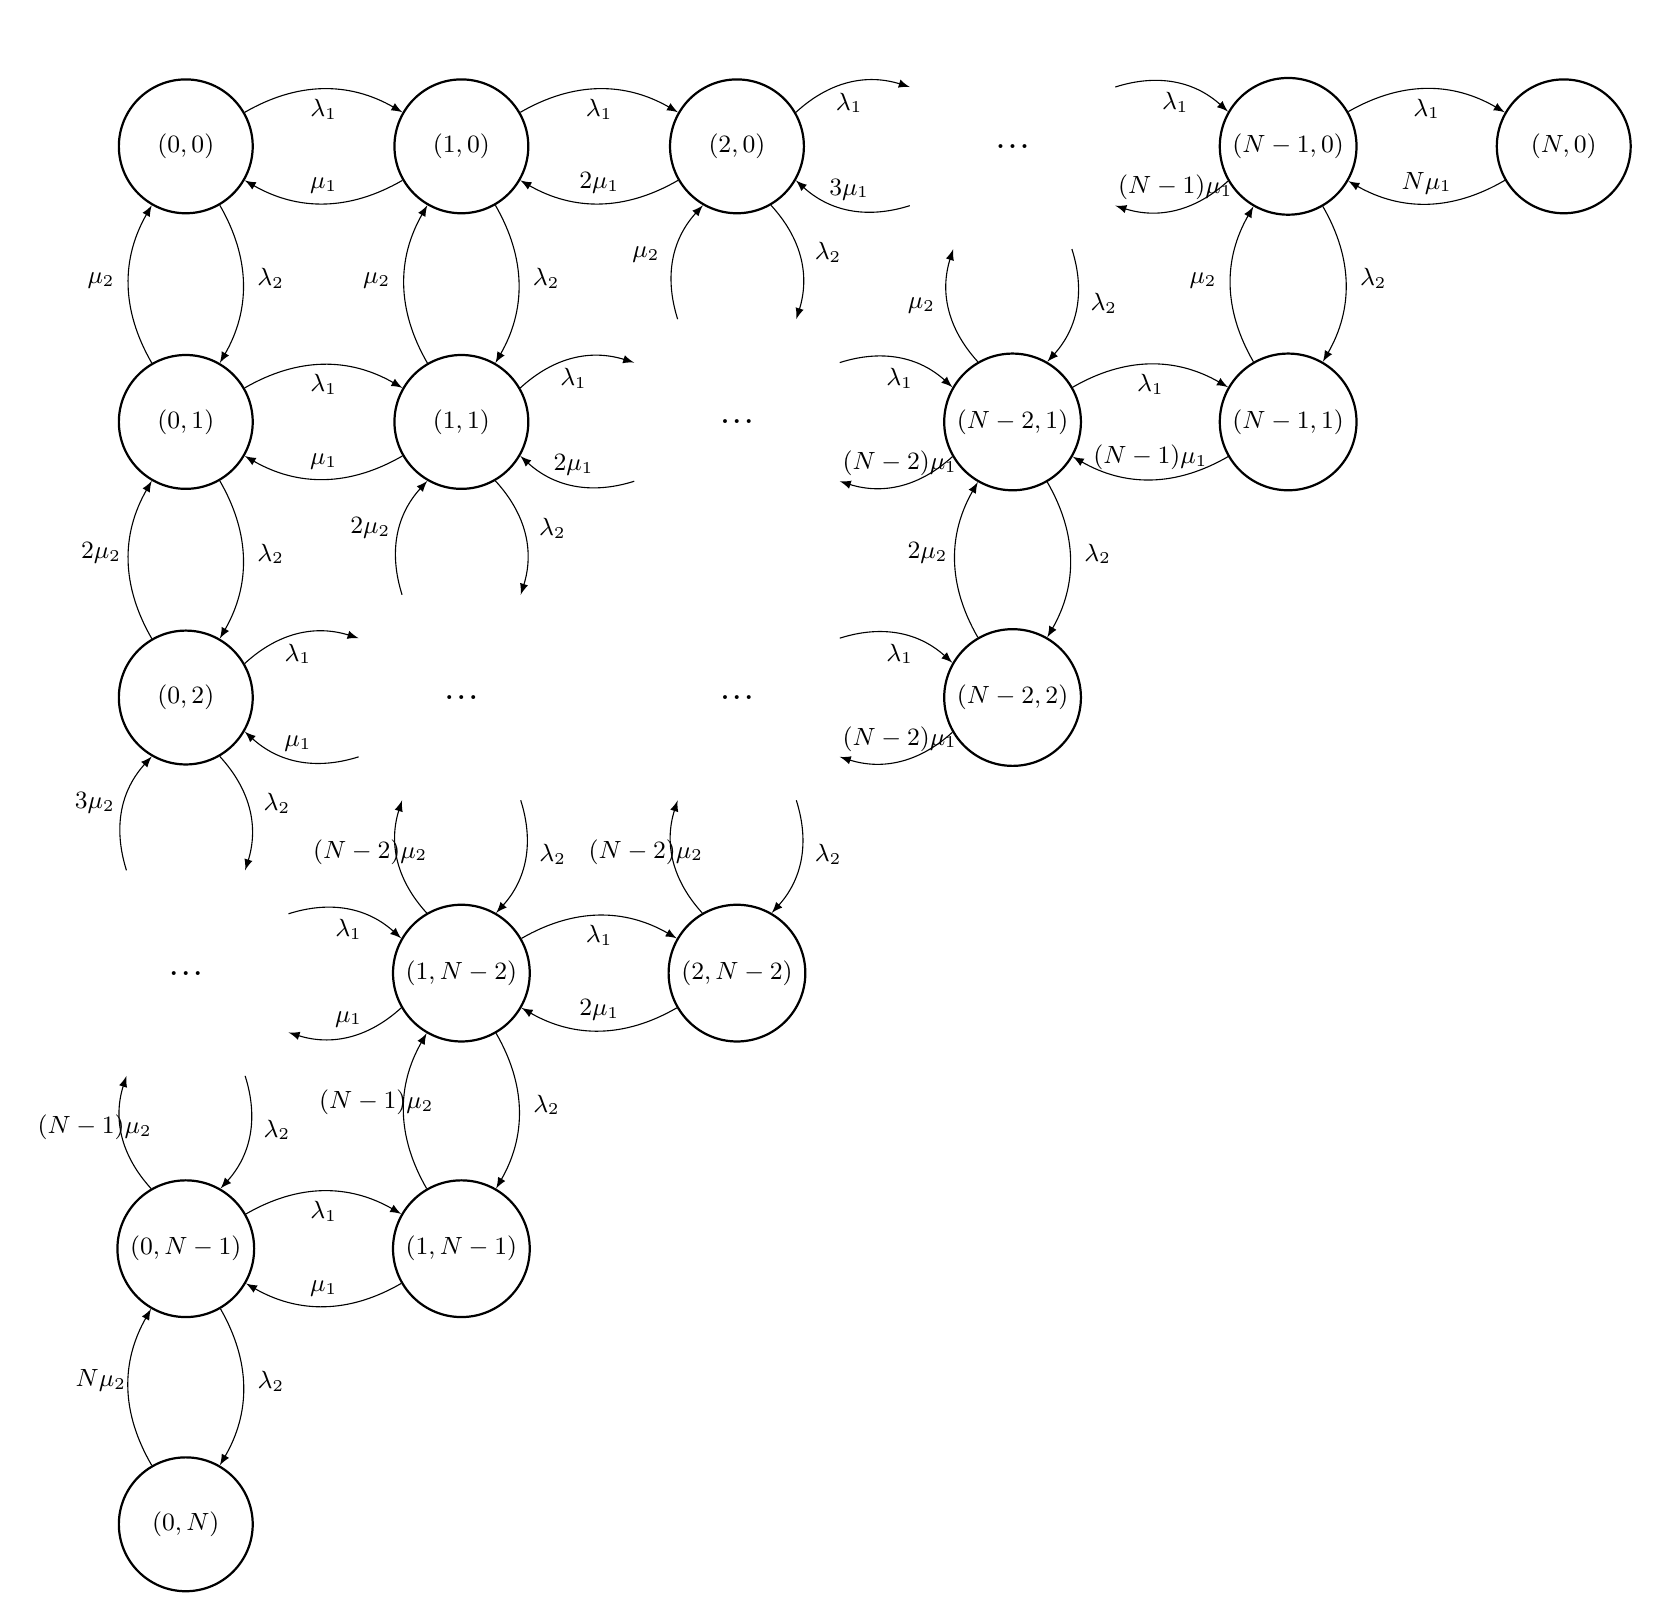
\begin{tikzpicture}[->,node distance=3.5cm,>=latex,font=\small, minimum width=1.7cm]

    \tikzstyle{round}=[thick,draw=black,circle]

    \node[round] 			    (00) {$(0,0)$};
    \node[round,right of=00]    (10) {$(1,0)$};
    \node[round,below of=00]    (01) {$(0,1)$};
    \node[round,below of=10]    (11) {$(1,1)$};
    \node[round,below of=01]    (02) {$(0,2)$};
    \node[round,right of=10]    (20) {$(2,0)$};
   
    \node[circle,draw=white,right of=20, minimum width = 3cm]    (A1) {\LARGE ...};
    \node[circle,draw=white,below of=02, minimum width = 3cm]    (A2) {\LARGE ...};
     
   	\node[round,right of=A1]    (N-1/0)  	{$(N-1,0)$};
   	\node[round,right of=N-1/0] (N0)	 	{$(N,0)$};
    \node[round,below of=N-1/0] (N-1/1)     {$(N-1,1)$};
    \node[round,left  of=N-1/1] (N-2/1)	{$(N-2,1)$};
    \node[round,below of=N-2/1] (N-2/2)	{$(N-2,2)$};
   
    \node[round,below of=A2]    (0/N-1)  	{$(0,N-1)$};
   	\node[round,below of=0/N-1] (0N)	 	{$(0,N)$};
    \node[round,right of=0/N-1] (1/N-1)     {$(1,N-1)$};
    \node[round,above of=1/N-1] (1/N-2)     {$(1,N-2)$};
    \node[round,right of=1/N-2] (2/N-2)	    {$(2,N-2)$};
    
    
    \node[circle,draw=white,left of=N-2/1,minimum width = 3cm]        (A3)     {\LARGE ...};
    \node[circle,draw=white,below of=11,minimum width = 3cm]          (A4)     {\LARGE ...};
    \node[circle,draw=white,above of=2/N-2,minimum width = 3cm]       (A5)     {\LARGE ...};
 
 
 	\path 
 	(00) 	edge[bend left,below]		node 					    {$\lambda_1$}		(10)
 		 	edge[bend left,above]       node [xshift=10,yshift=-5]  {$\lambda_2$} 		(01)
 	
 	(10) 	edge[bend left,above]       node 						{$\mu_1$} 			(00)
 		 	edge[bend left,below]		node 					    {$\lambda_1$}		(20)
 		 	edge[bend left,above]       node [xshift=10,yshift=-5]  {$\lambda_2$} 		(11)
 	
    (01) 	edge[bend left,above]       node [xshift=-10,yshift=-5] {$\mu_2$} 			(00)
   		 	edge[bend left,below]		node 					    {$\lambda_1$}		(11)
   	     	edge[bend left,above]       node [xshift=10,yshift=-5]  {$\lambda_2$} 		(02)
   
    (20) 	edge[bend left,above]       node 						{$2\mu_1$} 			(10)
    		edge[bend left,below]		node 					    {$\lambda_1$}		(A1)
    		edge[bend left,above]       node [xshift=10,yshift=-5]  {$\lambda_2$} 		(A3)
   		    
    (02) 	edge[bend left,above]       node [xshift=-10,yshift=-5] {$2\mu_2$} 			(01)
    		edge[bend left,above]       node [xshift=10,yshift=-5]  {$\lambda_2$} 		(A2)
    		edge[bend left,below]		node 					    {$\lambda_1$}		(A4)
   
    (11) 	edge[bend left,above]       node [xshift=-10,yshift=-5] {$\mu_2$} 			(10)
   		 	edge[bend left,above]       node 						{$\mu_1$} 			(01)
   		 	edge[bend left,below]		node 					    {$\lambda_1$}		(A3)
   		 	edge[bend left,above]       node [xshift=10,yshift=-5]  {$\lambda_2$} 		(A4)
   
   	(N0) 	edge[bend left,above]       node 						{$N\mu_1$} 			(N-1/0)
   
   	(N-1/0) edge[bend left,below]		node 					    {$\lambda_1$}		(N0)
   			edge[bend left,above]       node [xshift=10,yshift=-5]  {$\lambda_2$} 		(N-1/1)
   			edge[bend left,above]       node 						{$(N-1)\mu_1$} 			(A1)
   
    (N-1/1) edge[bend left,above]       node [xshift=-10,yshift=-5] {$\mu_2$} 			(N-1/0)
    		edge[bend left,above]       node 						{$(N-1)\mu_1$} 		(N-2/1)
    
    (N-2/1) edge[bend left,below]		node 					    {$\lambda_1$}		(N-1/1)
    		edge[bend left,above]       node [xshift=-10,yshift=-5] {$\mu_2$} 			(A1)
    		edge[bend left,above]       node 						{$(N-2)\mu_1$} 		(A3)
    		edge[bend left,above]       node [xshift=10,yshift=-5]  {$\lambda_2$} 		(N-2/2)
    		
    (N-2/2) edge[bend left,above]       node [xshift=-10,yshift=-5] {$2\mu_2$} 			(N-2/1)
    		edge[bend left,above]       node 						{$(N-2)\mu_1$} 		(A5)
    
    (0N) 	edge[bend left,above]       node [xshift=-10,yshift=-5]	{$N\mu_2$} 			(0/N-1)
   
   	(0/N-1) edge[bend left,below]		node 					    {$\lambda_1$}		(1/N-1)
   			edge[bend left,above]       node [xshift=10,yshift=-5]  {$\lambda_2$} 		(0N)
   			edge[bend left,above]       node [xshift=-10,yshift=-5]	{$(N-1)\mu_2$} 		(A2)
   
    (1/N-1) edge[bend left,above]       node 						{$\mu_1$}  			(0/N-1)
    	    edge[bend left,above]       node [xshift=-10,yshift=-5]	{$(N-1)\mu_2$} 		(1/N-2)
    
    (1/N-2) edge[bend left,above]       node 						{$\mu_1$}  			(A2)
    		edge[bend left,above]       node [xshift=10,yshift=-5]  {$\lambda_2$} 		(1/N-1)
    		edge[bend left,above]       node [xshift=-10,yshift=-5]	{$(N-2)\mu_2$} 		(A4)
    		edge[bend left,below]		node 					    {$\lambda_1$}		(2/N-2)
    		
    (2/N-2) edge[bend left,above]       node 						{$2\mu_1$}  		(1/N-2)
    		edge[bend left,above]       node [xshift=-10,yshift=-5]	{$(N-2)\mu_2$} 		(A5)
    
    (A1)    edge[bend left,above]       node 						{$3\mu_1$} 			(20)
    	    edge[bend left,below]		node 					    {$\lambda_1$}		(N-1/0)
    	    edge[bend left,above]       node [xshift=10,yshift=-5]  {$\lambda_2$} 		(N-2/1)
    	    
    (A2)	edge[bend left,above]       node [xshift=10,yshift=-5]  {$\lambda_2$} 		(0/N-1)
    		edge[bend left,above]       node [xshift=-10,yshift=-5]	{$3\mu_2$} 			(02)
    		edge[bend left,below]		node 					    {$\lambda_1$}		(1/N-2)
    		
    (A3)    edge[bend left,below]		node 					    {$\lambda_1$}		(N-2/1)
    		edge[bend left,above]       node [xshift=-10,yshift=-5]	{$\mu_2$} 			(20)
    		edge[bend left,above]       node 						{$2\mu_1$} 			(11)
    
    (A4)    edge[bend left,above]       node [xshift=-10,yshift=-5]	{$2\mu_2$} 			(11)
    		edge[bend left,above]       node 						{$\mu_1$} 			(02)
    		edge[bend left,above]       node [xshift=10,yshift=-5]  {$\lambda_2$} 		(1/N-2)
    		
    (A5)    edge[bend left,above]		node [xshift=10,yshift=-5]  {$\lambda_2$}		(2/N-2)
    		edge[bend left,below]		node 					    {$\lambda_1$}		(N-2/2);
   
\end{tikzpicture}
\end{adjustbox}
\end{figure}



\end{document}